\section{Feynman Diagrams and Dimensional Regularization}

\subsection{Finishing the 2-Point Function Calculation}
We discussed quite a bit in a quasi-heuristic way about different types of correlation functions - generic, connected, irreducible. These are things that are not particularly clearly explained in most textbooks out there. I have tried to explain it in the textbook, if the lecture discussion was a bit unweildy/difficult to follow.

For now we only require the beginning of the argument. The class of all Feynman diagrams is the sum of all irreducible Feynman diagrams (diagramatically pictured below):

\begin{center}
    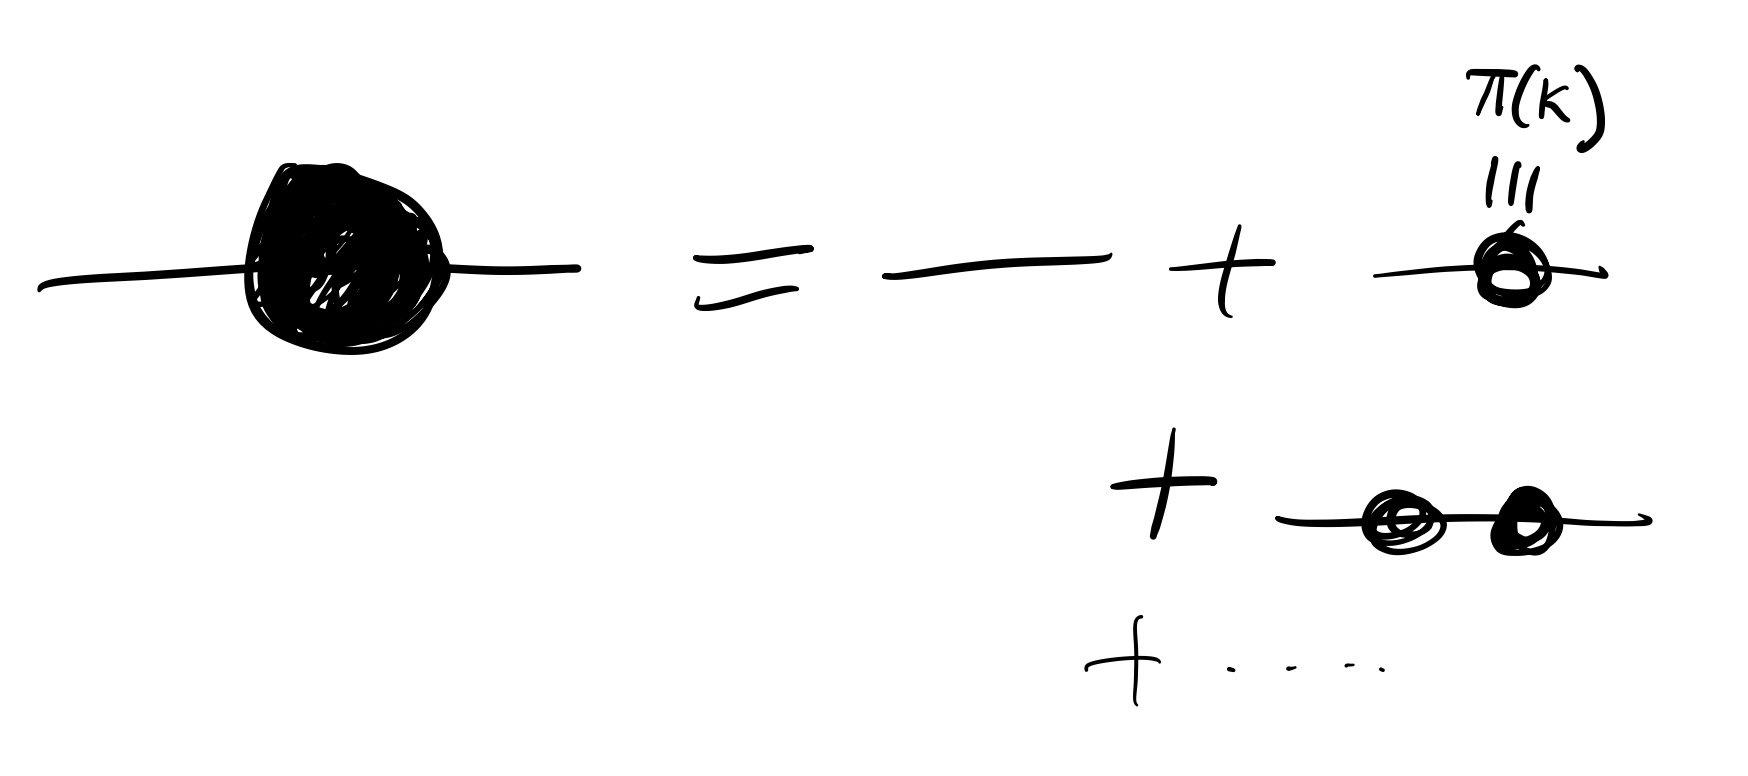
\includegraphics[scale=0.3]{Images/fig-lec28feynman1.png}
\end{center}


In momentum space, we had:
\begin{equation}
    D(k) = \Delta(k) + \Delta(k)\Pi(k)\Delta(k) + \Delta(k)\Pi(k)\Delta(k)\Pi(k)\Delta(k) + \ldots
\end{equation}
The only question left - are we sure of the values of the coefficient in the above expansion to be one? How do we figure that out? We could explore it by testing the diagrams, or systematically via generating functions.

Since the above is a geometric series, let us sum it up!
\begin{equation}
    \begin{split}
        D(k) &= \Delta(k)\left(1 + \Pi(k)\Delta(k) + (\Pi(k)\Delta(k))^2 + \ldots\right) 
        \\ &= \frac{\Delta(k)}{1 - \Pi(k)\Delta(k)} 
        \\ &=  \frac{\frac{-i}{k^2 + m^2 - i\e}}{1 - \Pi(k)\frac{-i}{k^2 + m^2 - i\e}}
        \\ &= \frac{-i}{k^2 + m^2 + i\Pi(k) - i\e}
    \end{split}
\end{equation}
This appears like a translation of the mass term, and it is therefore called the self-energy.

Our Feynman diagram calculation looks like:

\begin{center}
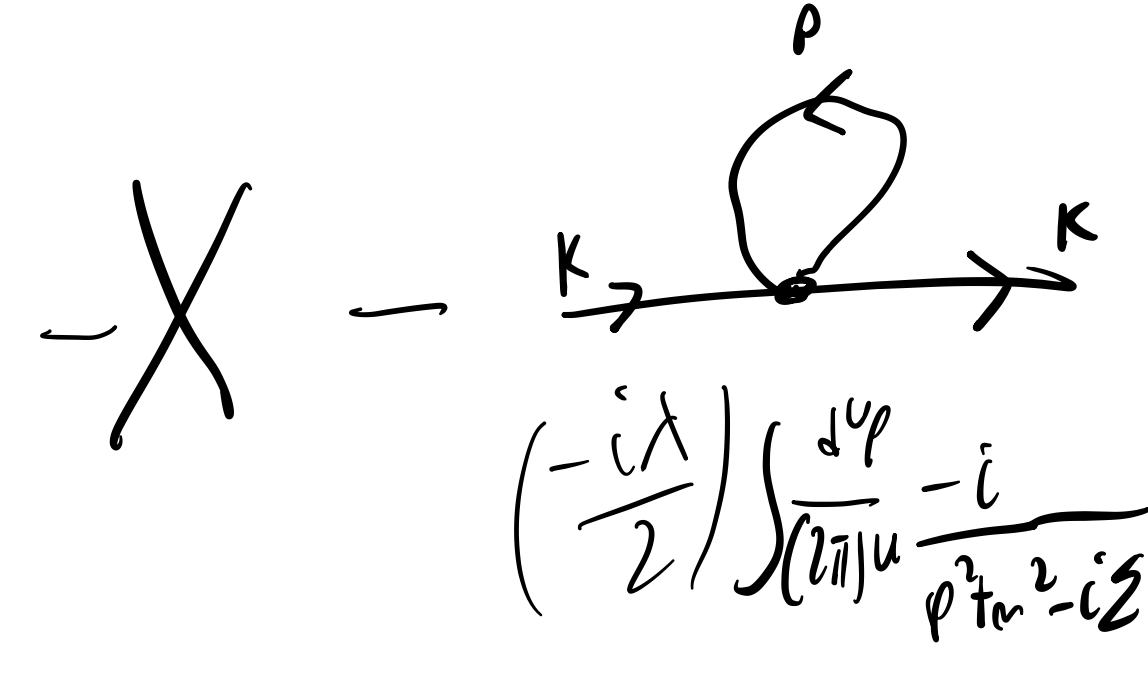
\includegraphics[scale=0.3]{Images/fig-lec28feynman2.png}
\end{center}

The extra factor of $i$ in the diagram with the loop term will make the correction imaginary, hence $i\Pi(k)$ will be real.

\subsection{4-Point Function}
We consider:
\begin{equation}
    \begin{split}
        \Gamma(x_1, \ldots x_n) = \bra{\O}T\varphi(x_1) \ldots \varphi(x_n)\ket{\O}
    \end{split}
\end{equation}
and we also have $\Gamma_C$ connected, $\Gamma_I$ irreducible. We will study the irreducible one as there is a lot of redundant information in the full four-point function. Let us however consider the combinatorics that allows us to cast the full four-point function in terms of the irreducible ones. We first have:
\begin{equation}
    \Gamma(x_1, \ldots, x_n) = \int \frac{d^4p_1}{(2\pi)^4}\ldots \frac{d^4p_n}{(2\pi)^4} e^{i(p_1x_1 + \ldots p_n x_n)}\Gamma(p_1, \ldots, p_n)(2\pi)^4 \delta(p_1 + \ldots p_n)
\end{equation}
Because of translation invariance, the $\Gamma$ on the LHS is equal to itself translated by some constant in space. So on the LHS we should have the conservation of momentum; hence the $\delta$ function appearing. Now consider writing a four-point $\Gamma$ as a bunch of connected terms:
\begin{equation}
    \begin{split}
        \Gamma(p_1, p_2, p_3, p_4) &= \Gamma(p_1, p_2)\Gamma(p_3, p_4) + \Gamma(p_1, p_3)\Gamma(p_2, p_4) + \Gamma_C(p_1, p_2, p_3, p_4) 
        \\ &= \Gamma_C(p_1, p_2)\Gamma_C(p_3, p_4) + \Gamma_C(p_1, p_3)\Gamma_C(p_2, p_4) + \Gamma_C(p_1, p_2, p_3, p_4)
    \end{split}
\end{equation}
where we note that $\Gamma(p_1, p_2) = \Gamma_C(p_1, p_2)$ for two-point functions - actually only specifically when $p_2 = -p_1$. So really, $\Gamma(p_1, -p_1) = \Gamma_C(p_1, -p_1) = D(p)$. So, if we know the two-point functions and the connected four-point function, we can plug them into the above. The irreducible ones are now a short reach away. 

The connected 4-point functions are ones with 4 legs sticking out. We make it reducible by adding something to one of the legs. If we factor our those things, what is left in the middle is irreducible.

\begin{center}
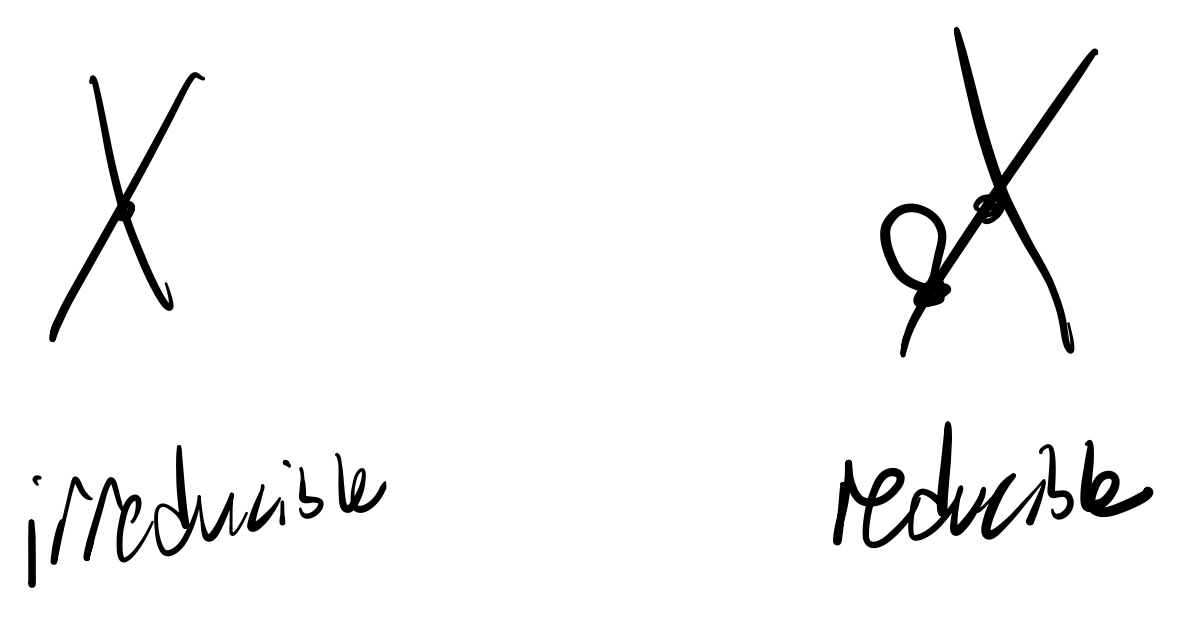
\includegraphics[scale=0.3]{Images/fig-lec28feynman3.png}
\end{center}

This tells me that:
\begin{equation}
    \Gamma_C(p_1, p_2, p_3, p_4) = D(p_1)D(p_2)D(p_3)D(p_4)\Gamma(p_1, p_2, p_3, p_4)
\end{equation}

So if I compute two-point functions and the irreducible four-point function to some order, I get the connected four-point function, which I can then get the full four-point function from. This is all easy algebra - no integrals!

Tadpole Diagram - here is a diagram we considered before:

\begin{center}
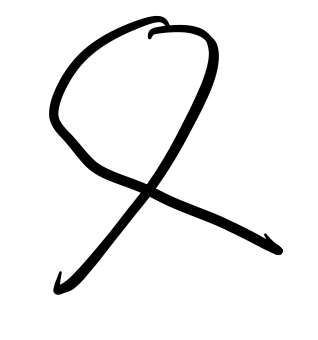
\includegraphics[scale=0.3]{Images/fig-lec28feynman4.png}
\end{center}

But this is reducible; so the lines present are not actually real lines.

Ok, let's now calculate the irreducible 4-point function, as from it we can reconstruct what we already know. Let us start drawing some Feynman diagrams. If I have zero vertices, what I have is neither irreducible, nor connected.

\begin{center}
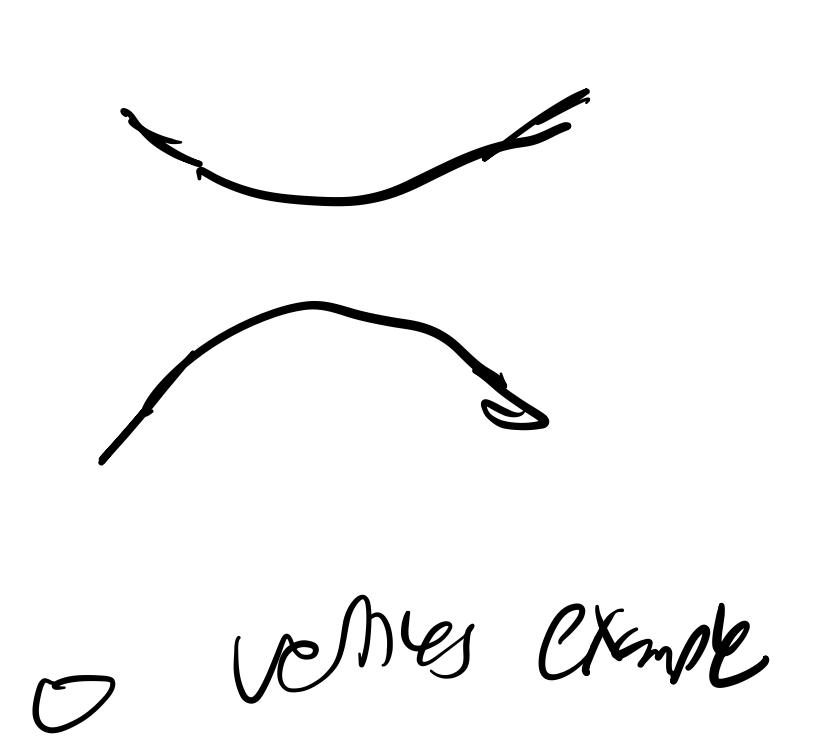
\includegraphics[scale=0.3]{Images/fig-lec28feynman5.png}
\end{center}

So our irreducible 4-point function begins at some power of $\lambda$. For $\lambda^1$, we have that the only way to get something irreducible is for the external legs to all connect with the vertex:

\begin{center}
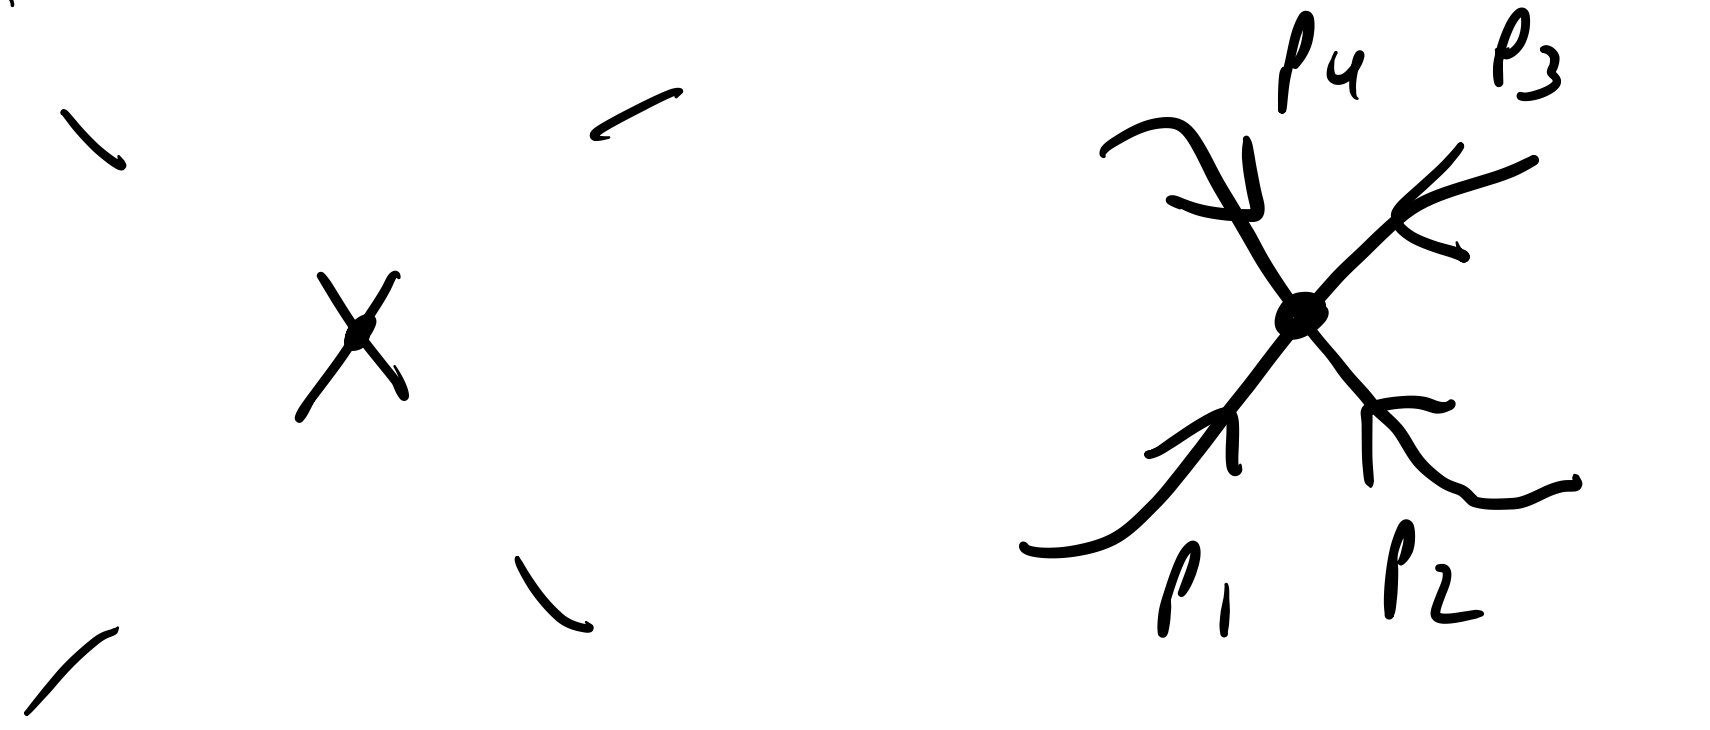
\includegraphics[scale=0.3]{Images/fig-lec28feynman6.png}
\end{center}

But there are 4 choices for the first leg, 3 for the second, 2 for the third, and one for the fourth, so we have a weight $\frac{-i}{4!}\lambda 4 \cdot 3 \cdot 2 \cdot 1 = -i\lambda$. So:
\begin{equation}
    \Gamma_I(p_1, p_2, p_3, p_4) = -i\lambda
\end{equation}
so this captures the interaction in the sense that it just produces the coupling constant! It is independent of the $p$s - as it is a pointlike interaction (the only thing being important is that the net momenta is zero).

Now, let's consider the next order - this should give the quantum corrections to the interaction (the first order result is really just what classical field theory would have told us). We go to $\lambda^2$. Our overall factor is $\frac{1}{2!}\left(\frac{-i\lambda}{4!}\right)^2$. We are only interested in the irreducible diagrams. The first line has to go to a vertex (and not another external leg), and we have $8$ choices for where it could go. Now, there's a couple of choices. It can't go to one of the external legs, but it can go to either the first or the second vertex - there will be two classes. Let's consider the class where it goes to the first vertex. Next, I have to attach the remaining two legs. If I attach the remaining external legs to the first vertex, then the diagram is reducible; this is because then the remaining leg from the first vertex will have to connect to the other part of the diagram, and this can be cut to form two diagrams. So, there are four choices (on the second vertex) for the third leg, and three choices for the fourth leg. Now, there are two ways to pair up the four remaining legs from the vertices in a way that connects the two diagrams. So, the counting gives $\frac{1}{2!}\left(\frac{-i\lambda}{4!}\right)^2 \cdot 8 \cdot 3 \cdot 4 \cdot 3 \cdot 2$.

\begin{center}
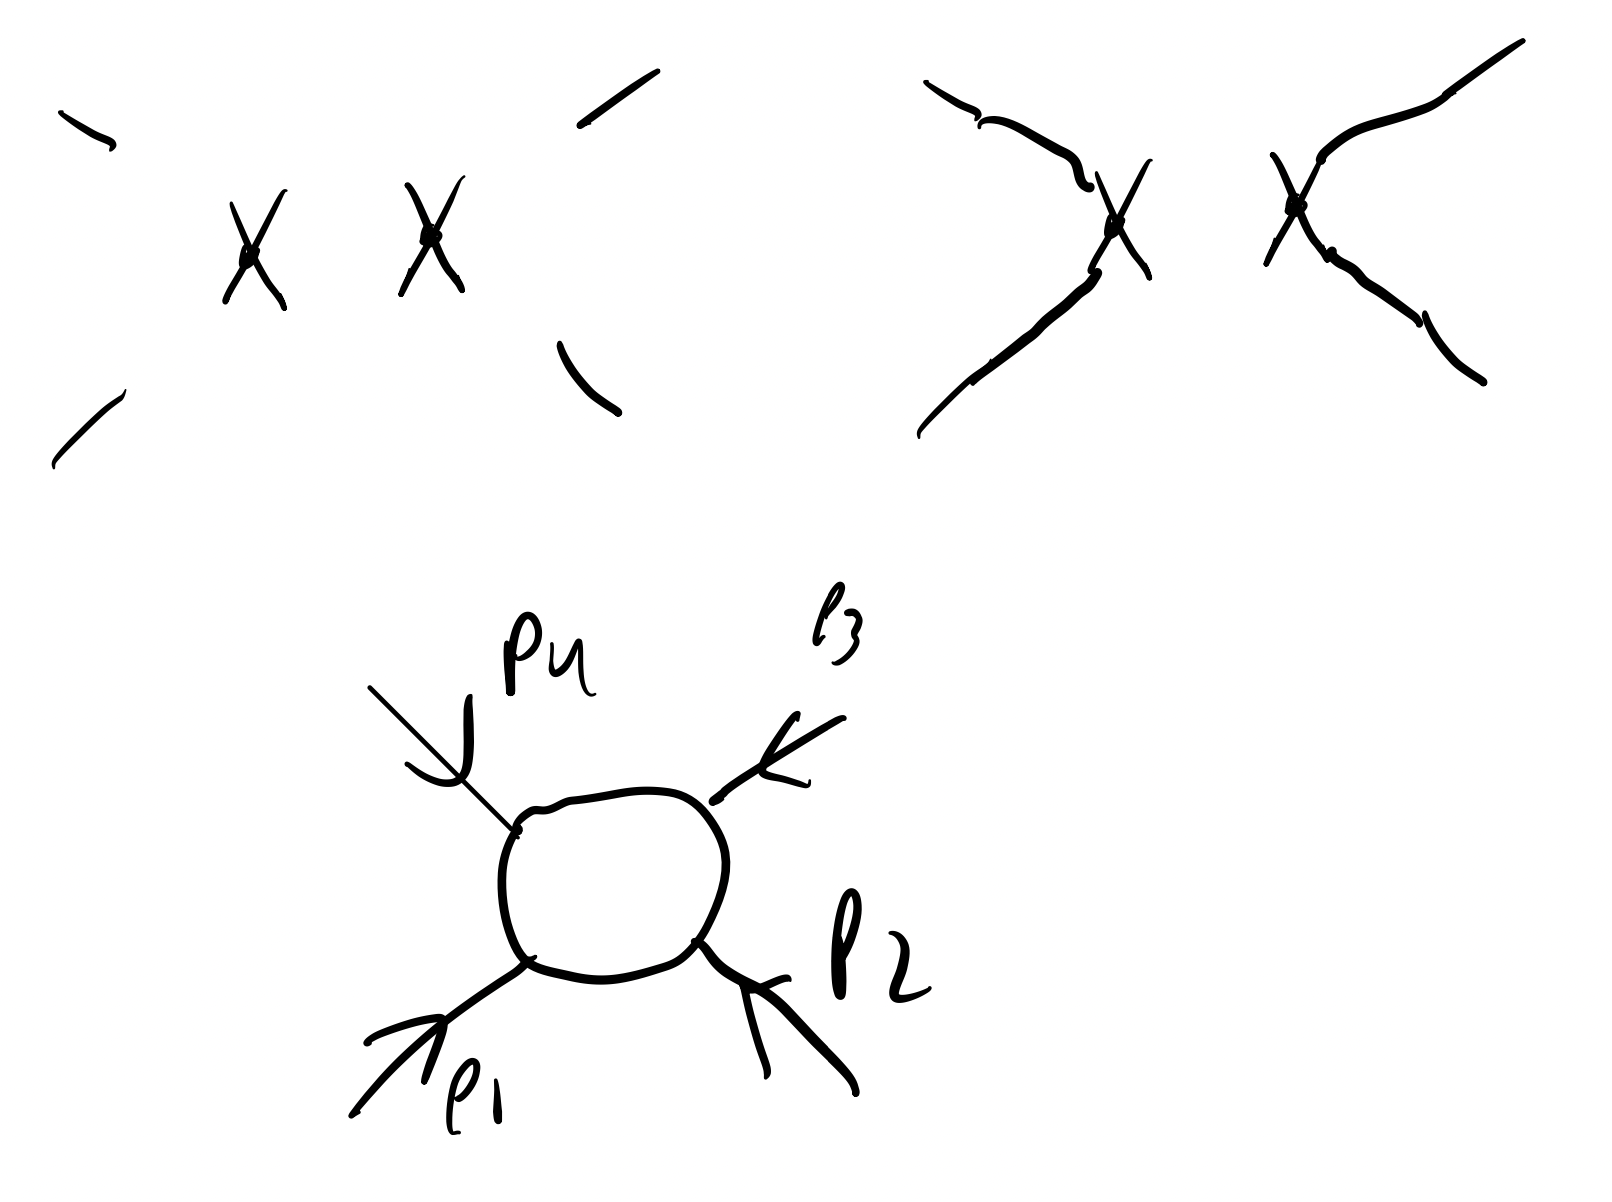
\includegraphics[scale=0.3]{Images/fig-lec28feynman7.png}
\end{center}

the other classes of possible diagrams look like:

\begin{center}
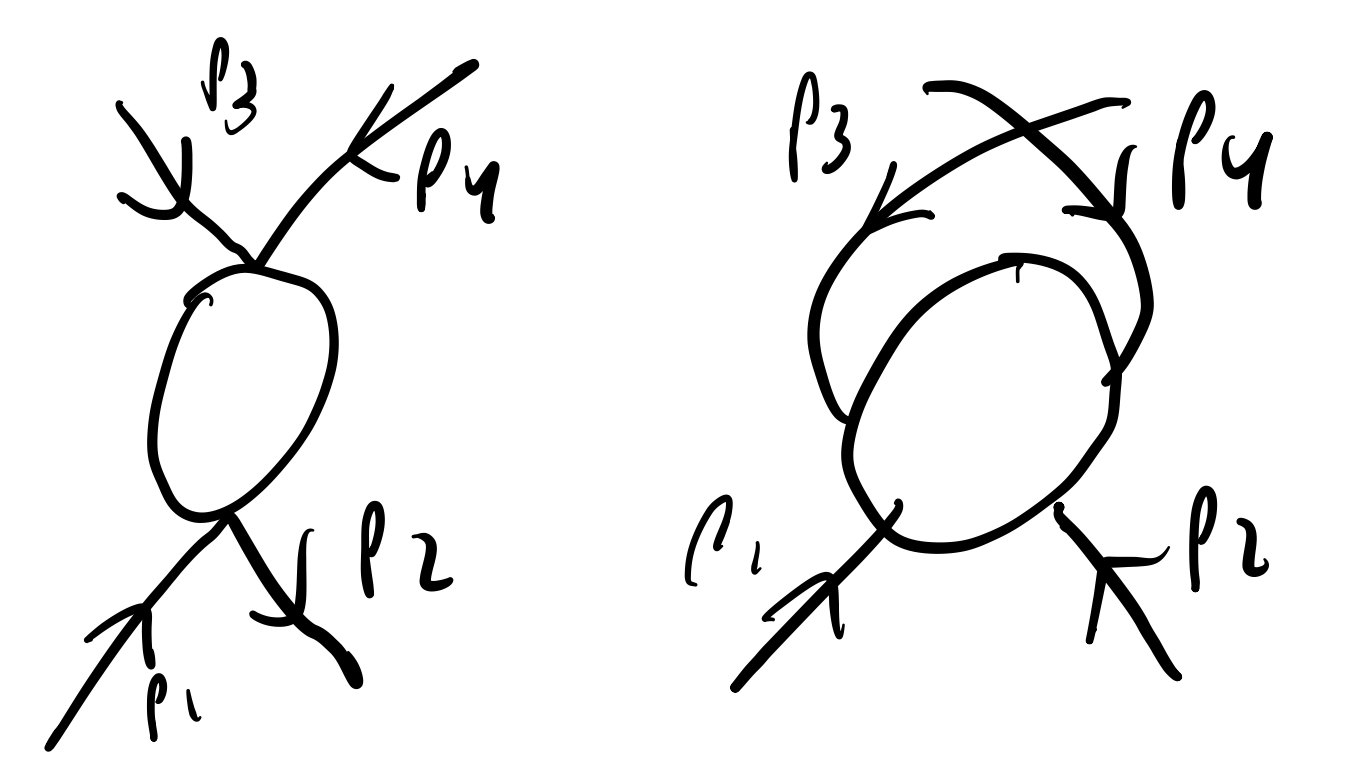
\includegraphics[scale=0.3]{Images/fig-lec28feynman8.png}
\end{center}

So we have three classes of diagrams, each with the same multiplicity, so overall the weight is $\frac{\lambda^2}{2}$. Now we have to go back to the analytic expressions, and recall what to put in. In momentum space this is very doable. Just put things into the diagram, and integrate over the remaining free momenta - of which there should be one per closed loop in the diagram (e.g. one momentum $q$ for the one-loop diagrams we consider here).

\begin{center}
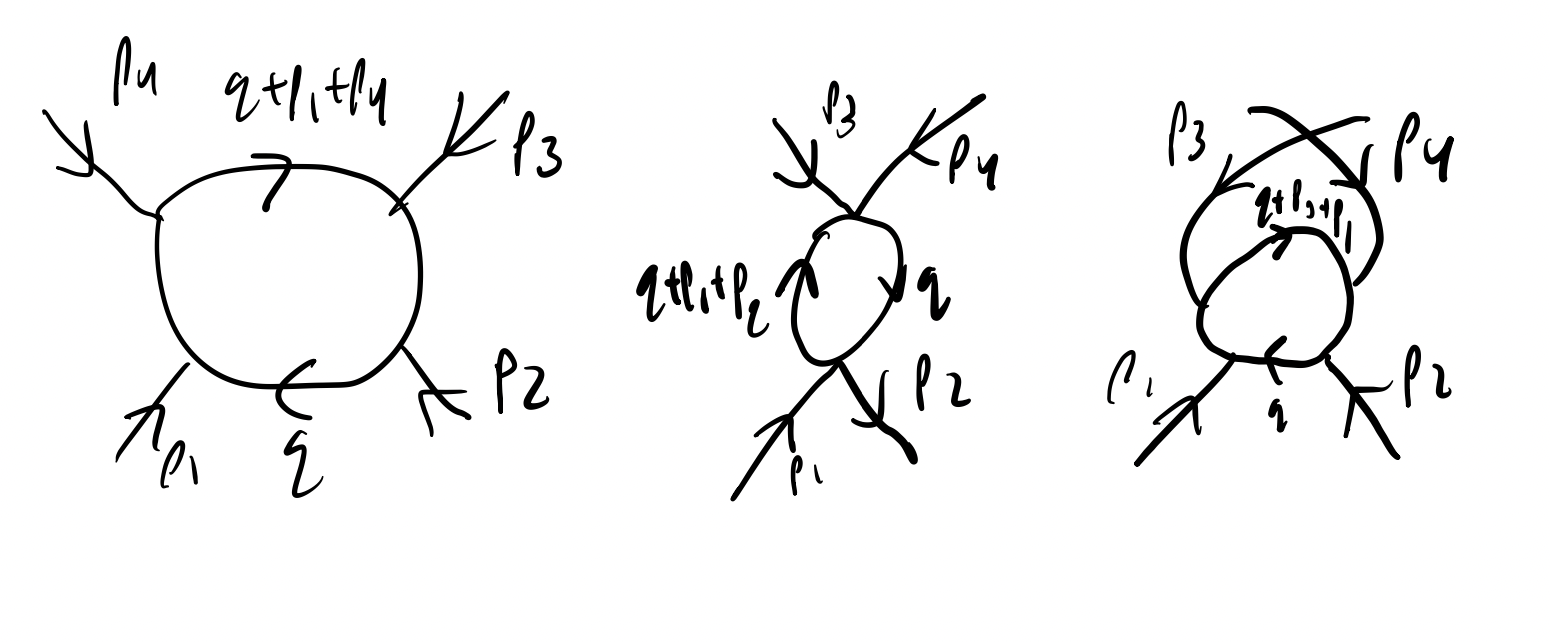
\includegraphics[scale=0.3]{Images/fig-lec28feynman9.png}
\end{center}

So our expression is:
\begin{equation}
    \begin{split}
        \Gamma_I(p_1, p_2, p_3, p_4) &= -i\lambda + \frac{\lambda^2}{2}\int \frac{d^4q}{(2\pi)^4}\Delta(q)\Delta(q + p_1 + p_4) 
        \\ &+ \frac{\lambda^2}{2}\int \frac{d^4q}{(2\pi)^4}\Delta(q)\Delta(q + p_1 + p_2) + \frac{\lambda^2}{2}\int \frac{d^4q}{(2\pi)^4}\Delta(q)\Delta(q + p_1 + p_3) + O(\lambda^3)
    \end{split}
\end{equation}
so we must consider the integral:
\begin{equation}
    I(p) = \frac{\lambda^2}{2}\int \frac{d^4q}{(2\pi)^4}\frac{-i}{q^2 + m^2 - i\e} \frac{-i}{(q+p)^2 + m^2 - i\e}
\end{equation}
but this diverges (logarithmically). So we must do something to make this sensible - regularization. 

\subsection{Dimensional Regularization}
This has a long history and there is all sorts of tricks one can do, but they all amount to modifying this integral somehow such that the integral becomes by finite. We could for example replace $\Delta$ by some other function, and then we remove this modification later on. We could also put just an upper cutoff onto $q$. This is legitimate, but a little bit clumsy, as the translation invariance of the $q$ of the integral is messed up by the cutoff momenta (though for logarithmic divergences, it doesn't mess it up in a very terrible way). We do the easiest fix up here, though logically the least transparent. We assume that we are not really in 4-dimensions, but in some other spacetime dimension, calculate the integral with that dimension by some parameter, and then analytically continue the result to four-dimension. This is known as \emph{dimensional regularization}. Historically, it was important as it is a regularization that does not violate very many symmetries. In the literature, this is basically the only method used. 

Note that we generally wish to expand in a dimensionless constant (e.g. $\lambda$). We therefore add a constant with dimensions of mass to compensate for the modified dimensionality of the integral:
\begin{equation}
    I(p) = \frac{\lambda^2}{2}\mu^{4 - 2w}\int \frac{dq^{2w}}{(2\pi)^{2w}} \frac{-i}{q^2 + m^2 - i\e} \frac{-i}{(q+p)^2 + m^2 - i\e}
\end{equation}
Even without have to introduce a explicit cutoff, we have had to introduce an explicit scale here. Now, we can assume $w$ sufficiently small such that the integral will converge.

We will now simplify the formula using Feynman parameters:
\begin{equation}
    \frac{1}{AB} = \int_0^1 d\alpha \frac{1}{(\alpha A + (1-\alpha)B)^2}
\end{equation}
In the textbook there is a more general formula of the above. Why would I do this (introduce more integrals!?) - this is because this will allow us to combine the denominators. Our integral becomes:
\begin{equation}
    I(p) = -\frac{\lambda^2\mu^{4-2w}}{2}\int_0^1 d\alpha \int \frac{d^{2w}q}{(2\pi)^{2w}} \frac{1}{(q^2 + p^2\alpha(1-\alpha) + m^2 - i\e)^2}
\end{equation}
Note that we have translated $q$ so as to get rid of a cross-term in the denominator. I could evaluate this via Cauchy's integral, but there would be some symmetry violations. Instead, we do a Rick rotation. We write the integral of $q_0$ which is along the real axis (blue, below) as a sum along the imaginary axis (red) plus a ``figure-eight'' type contour (purple). 

\begin{center}
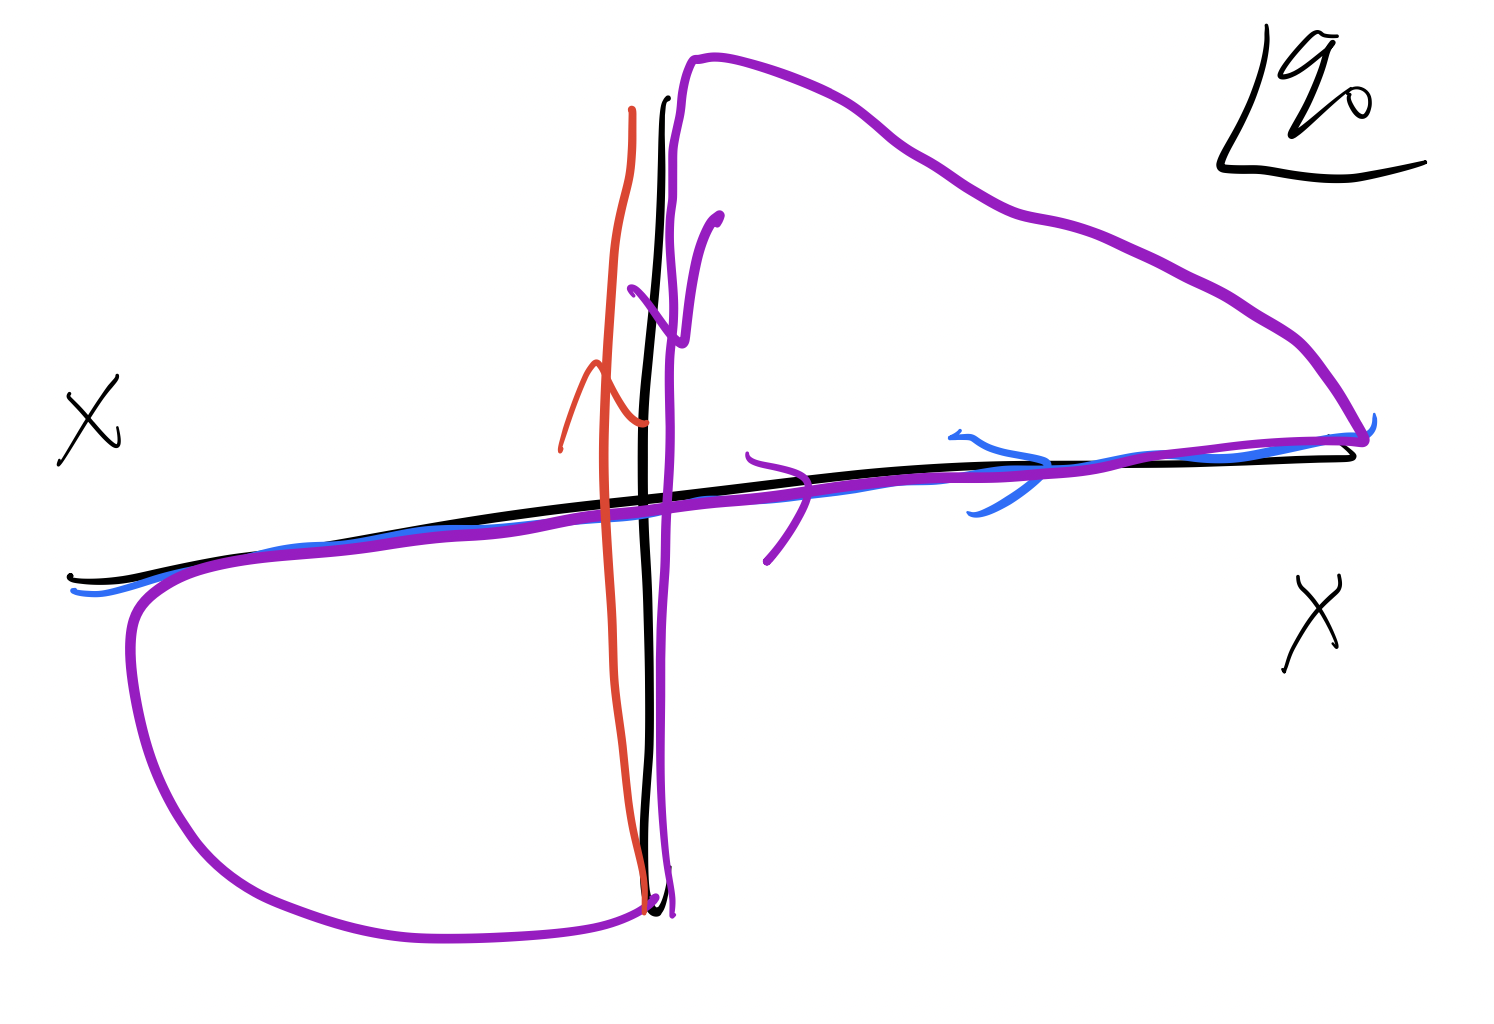
\includegraphics[scale=0.3]{Images/fig-lec28integral.png}
\end{center}

We change variables $q_0 \to iq_0, p_0 \to ip_0$:
\begin{equation}
    I(p) = -\frac{i\lambda^2 \mu^{4-2w}}{2}\int_0^1d\alpha \int \frac{d^{2w}q}{(2\pi^2)}\frac{1}{(q^2 + p^2\alpha(1 - \alpha)m^2)^2}
\end{equation}
We discuss how to carry this out next day, but we give the result today:
\begin{equation}
    I(p) = -\frac{i\lambda^2\mu^{4 - 2w}}{2}\int_0^1 d\alpha \frac{\Gamma(2 - w)}{(4\pi)^w} \frac{1}{(p^2\alpha(1-\alpha) + m^2)^{2-w}}
\end{equation} 
The last integral is an unelightening hypergeometric type deal, so we leave it as an integral. Note that we have now $I$ as a function of the dimensionality $w$. There, the Gamma-function diverges: $\Gamma(2 - w) = \frac{1}{2-w} + \gamma + \ldots$. So this is now where the divergence is hiding. We still have to do something about it - but we now have it in a form where it is understandable. The next step will be to do an asymptotic expansion in 4-dimensions, and isolate the divergent and non-divergent part. This would give us the answer.

We've just done a one-loop integral. This kind of integral we will see again a few times, and the technique for computing it is more or less the same in all cases.